\section {Development Timeline}

	We use Gantt Charts as graphical representations of all the tasks that are needed for the completion of the project. The Gantt Chart proves to be an efficient visual method of tracking the different tasks of the project and helps staying on schedule. For this report, we have only included tasks to which the computer engineers are specifically assigned.

\begin{figure}[H]
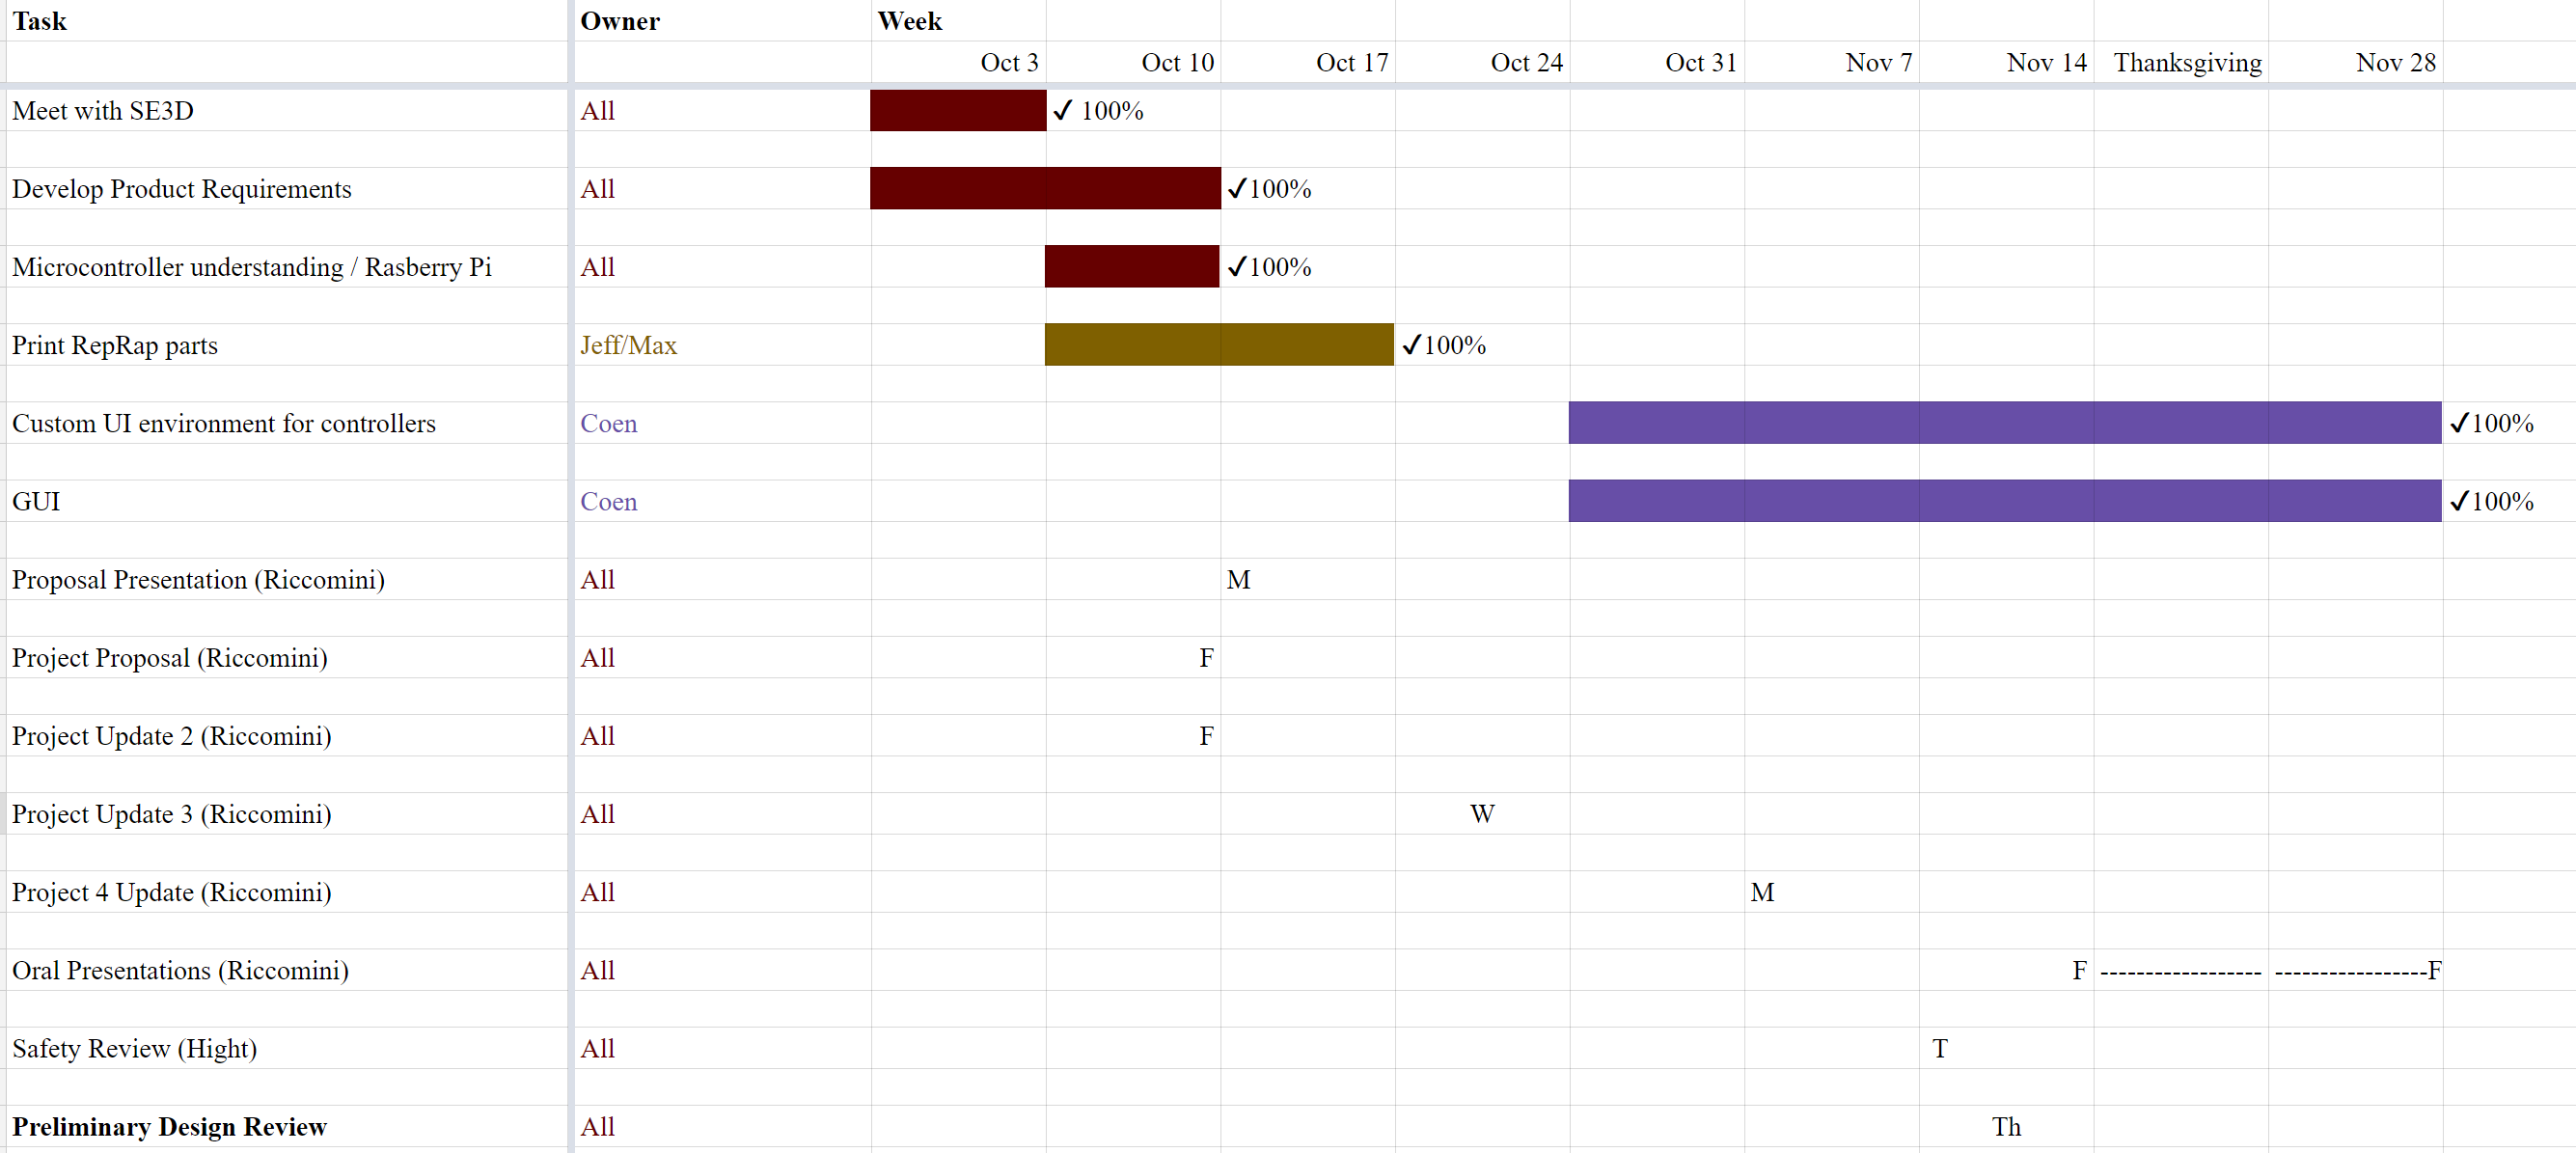
\includegraphics[scale=0.45]{gantt-fall}
\caption{\label{figure:gantt-fall} Fall Gantt Chart}
\end{figure}

\begin{figure}[H]
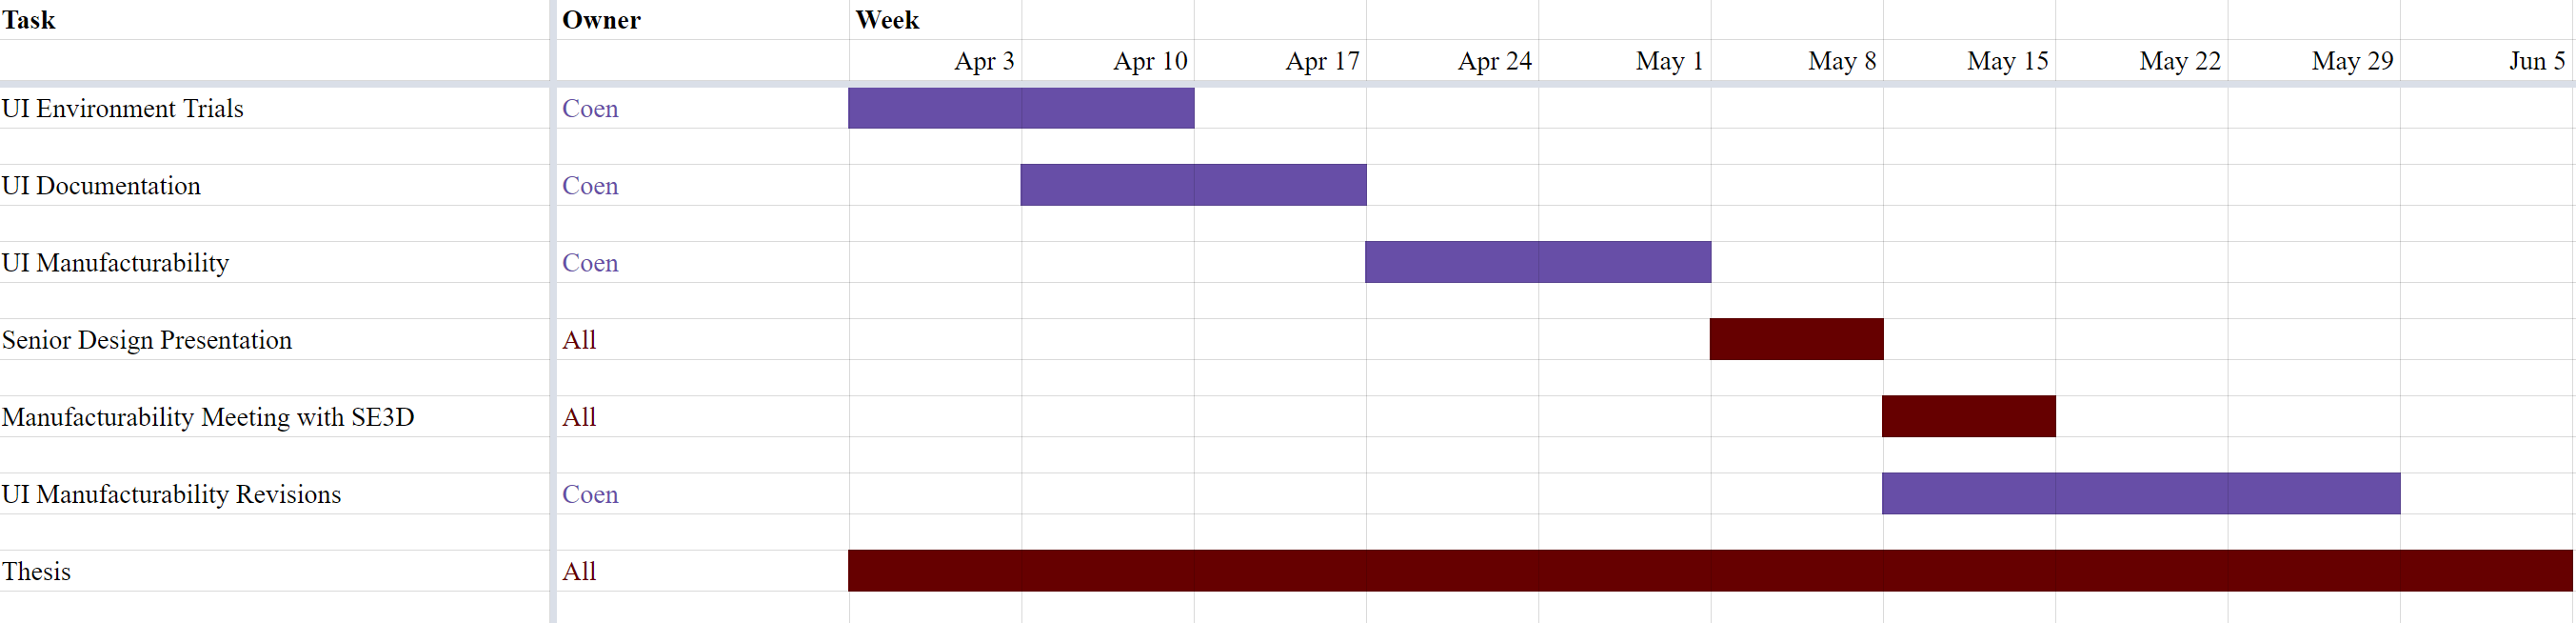
\includegraphics[scale=0.45]{gantt-winter}
\caption{\label{figure:gantt-winter} Winter Gantt Chart}
\end{figure}


\begin{figure}[H]
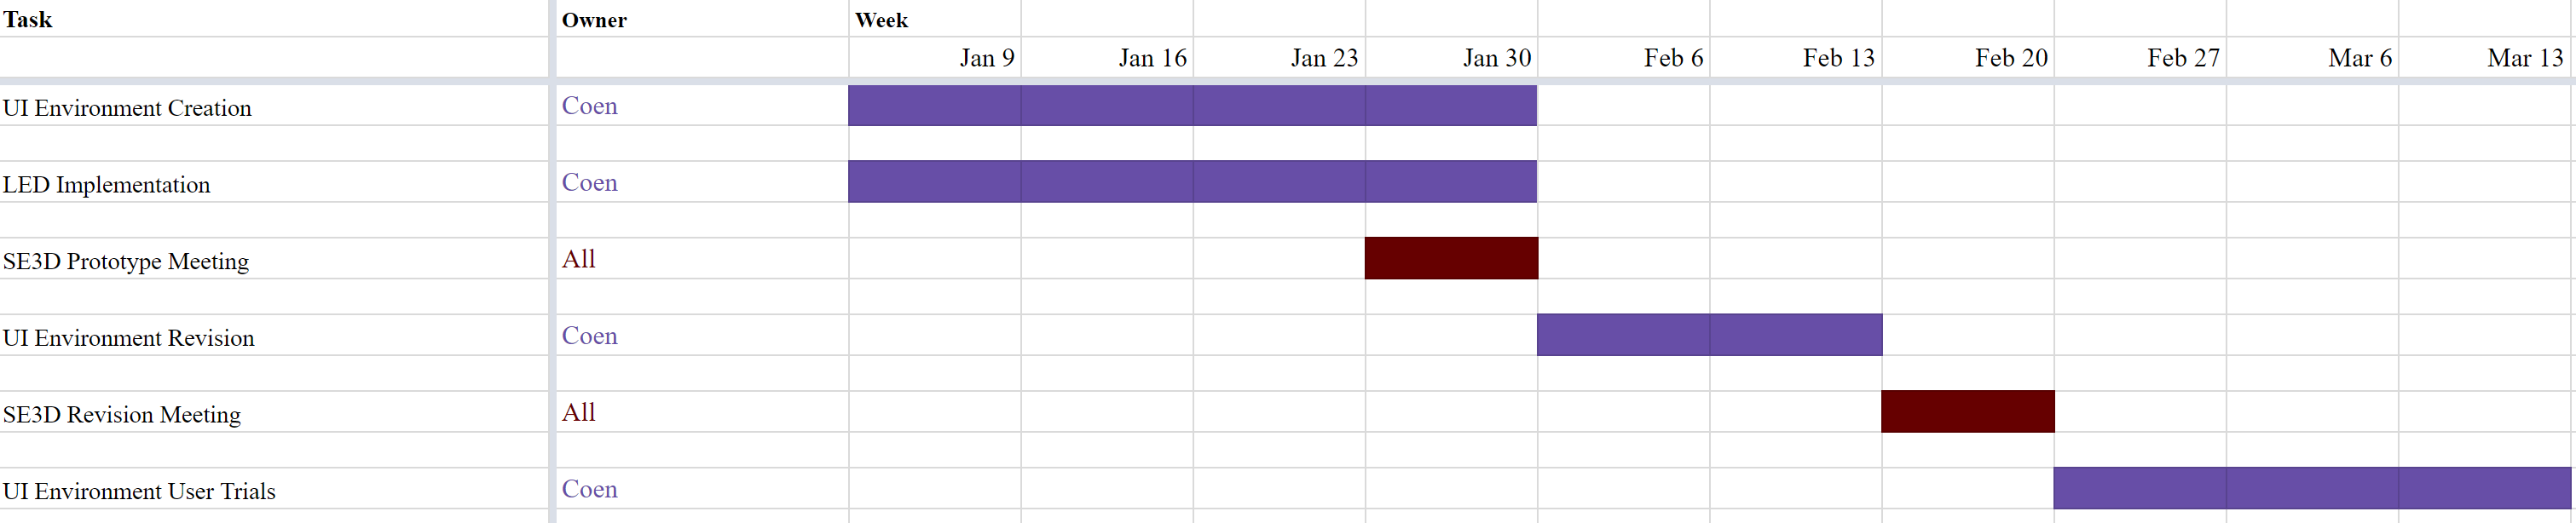
\includegraphics[scale=0.42]{gantt-spring}
\caption{\label{figure:gantt-spring} Spring Gantt Chart}
\end{figure}